\documentclass[12pt,letterpaper]{article}
%\usepackage[longnamesfirst]{natbib}
\usepackage[round]{natbib}
\usepackage{rotating}
\usepackage{cancel}
%\usepackage{appendix}
%\usepackage[toc,page]{appendix}
\usepackage{amsfonts,mathtools,amsmath}
\usepackage{setspace}
\usepackage{threeparttable}
\usepackage{amsmath}
\usepackage{amsfonts}
%\usepackage{natbib}
\usepackage{longtable,lscape}
\usepackage{amssymb}
\usepackage{graphicx} 
%\usepackage{indentfirst}
\usepackage{color}
\usepackage{float}
\usepackage[center]{caption}
\usepackage{subfigure}
\usepackage{plain}
%\usepackage{afterpage}
%\bibliographystyle{apsr}
\usepackage{theorem}
\usepackage{multirow,dcolumn,booktabs}
\usepackage{sectsty}
\usepackage{url}
\usepackage{chngcntr}
%\usepackage[capposition=top]{floatrow}
\sectionfont{\normalsize}
\subsectionfont{\normalsize}
\makeatletter
\renewcommand\thesubsection{\thesection.\@arabic\c@subsection}
\renewcommand\thesubsubsection{\thesubsection.\@arabic\c@subsubsection}
\makeatother

\setlength{\textwidth}{16cm} \setlength{\textheight}{22.8cm}
\addtolength{\oddsidemargin}{-13mm} \addtolength{\topmargin}{-10mm}
\setlength{\topmargin}{-.5in}
    \linespread{1.5}

\renewcommand{\labelenumii}{\arabic{enumi}}
\newcommand\independent{\protect\mathpalette{\protect\independenT}{\perp}}
\def\independenT#1#2{\mathrel{\rlap{$#1#2$}\mkern2mu{#1#2}}}

\DeclareMathOperator*{\rk}{rk}
\DeclareMathOperator*{\Card}{Card}
\DeclareMathOperator*{\Prob}{Prob}
\DeclareMathOperator*{\cov}{cov}
\DeclareMathOperator*{\var}{var}
\DeclareMathOperator{\Var}{Var\,}
\DeclareMathOperator{\Post}{Post}
\DeclareMathOperator{\Pre}{Pre}
\DeclareMathOperator{\post}{post}
\DeclareMathOperator{\pre}{pre}
\DeclareMathOperator{\Mid}{Mid}
\DeclareMathOperator{\MID}{MID}

\usepackage{float}
\usepackage{graphicx}
\graphicspath{{./graphics/}}
\usepackage[all]{nowidow}
\usepackage{multirow}
\usepackage{textcomp}
\usepackage{soul}

\usepackage{colortbl}
\usepackage{booktabs}
\usepackage{ragged2e}
\usepackage{threeparttable}
\newcommand{\tabnote}[1]{\vskip5pt{\justifying\noindent\small {\emph{Note:~}#1\par}}}
\usepackage{epigraph}
\usepackage{fullwidth}
\usepackage{fancyvrb} % Allows customization of verbatim environments
\fvset{fontsize=\normalsize}

% Coding stuff
\usepackage{placeins}
\newcommand{\codeexample}[2]{
	\begin{fullwidth}[width=\textwidth]
		\VerbatimInput[framesep=3mm,
			frame=lines, %line above and below code section
			numbers=left, %Line number
			label= #1, %name of code section
			baselinestretch=0.75 %Use line space more similar to line space in code editors
		]{#2} %Write the relative file path and the name of the file  to be included
	\end{fullwidth}
	\FloatBarrier
}


\begin{document}

\documentclass{book}
\usepackage{graphicx}


\begin{document}

Sergio Andrés García Bernal \hspace{1}
Causal Inference and Research Design \hspace{1}
Assignment 4: Sunday, June 14th, 2020


1.	
https://github.com/SergioGarcia211/RDD.git

2.	Summary Hansen’s paper
In this paper Hansen wants to test whether the harsher punishments and sanctions offenders experience at the BAC thresholds are effective in reducing drunk driving. The main idea is to find the causal effect of having a BAC above either 0.08 or 0.15 threshold on recidivism within four years of the original test. To carry out his work he uses the administrative records on 512,964 DUI stops in the state of Washington from 1995 to 2001, given that the BAC thresholds are constant since January 1, 1999, he encloses the data from 1999 to 2007. And taking advantages of the specific cutoffs for DUI and aggravated DUI, it allows the usage of a regression discontinuity design as the identification strategy.
The results suggest that harsher punishments and sanctions associated with BAC limits reduce future drunk driving. Finding evidence that having a BAC above either the 0.08 DUI threshold or the 0.15 aggravated DUI is associated with reduced repeat drunk driving both in the short and long term. In terms of elasticity: he found evidence that 10 percent increase in sanctions and punishments is associated with a 2.3 percent decline in drunk driving. Having a BAC above the DUI threshold decreases the probability of repeating the crime. 
3.	Do-file
4.	
The histogram of Figure 1 (recreated here) shows us the distribution of the blood alcohol content (BAC) tests. We can see little evidence of non-random heaping which means no evidence of manipulation of the running variable. But for going further we can use a test to check for this, it’s the McCrary Density test under the null hypothesis the density should be continuous at the cutoff point versus the alternative where the density should increase at the kink. Hansen has done it and has found a p-value of 0.59 for the 0.008 threshold, it is not possible rejecting, so he concludes there is no evidence of manipulation.


\begin{figure}
  \centering
    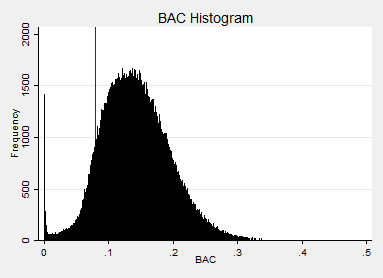
\includegraphics[width=0.7\textwidth]{Graph}
  \caption{Figure 1}

\end{figure}

\begin{table}[htbp]\centering
\def\sym#1{\ifmmode^{#1}\else\(^{#1}\)\fi}
\caption{Table 2 - Panel A}
\begin{tabular}{l*{4}{c}}
\hline\hline
            &\multicolumn{1}{c}{(1)}&\multicolumn{1}{c}{(2)}&\multicolumn{1}{c}{(3)}&\multicolumn{1}{c}{(4)}\\
            &\multicolumn{1}{c}{male}&\multicolumn{1}{c}{white}&\multicolumn{1}{c}{aged}&\multicolumn{1}{c}{acc}\\
\hline
1.DUI       &      0.0307\sym{***}&     0.00271         &      -7.787\sym{***}&      -0.219\sym{***}\\
            &   (0.00729)         &   (0.00617)         &     (0.204)         &   (0.00627)         \\
\hline
\(N\)       &      214558         &      214558         &      214558         &      214558         \\
\hline\hline
\multicolumn{5}{l}{\footnotesize Standard errors in parentheses}\\
\multicolumn{5}{l}{\footnotesize \sym{*} \(p<0.05\), \sym{**} \(p<0.01\), \sym{***} \(p<0.001\)}\\
\end{tabular}
\end{table}


\begin{table}[htbp]\centering
\def\sym#1{\ifmmode^{#1}\else\(^{#1}\)\fi}
\caption{Table 3 - Panel A}
\begin{tabular}{l*{3}{c}}
\hline\hline
            &\multicolumn{1}{c}{(1)}&\multicolumn{1}{c}{(2)}&\multicolumn{1}{c}{(3)}\\
            &\multicolumn{1}{c}{recidivism}&\multicolumn{1}{c}{recidivism}&\multicolumn{1}{c}{recidivism}\\
\hline
1.DUI       &     -0.0266\sym{***}&     -0.0549\sym{***}&       0.108         \\
            &   (0.00404)         &    (0.0152)         &    (0.0844)         \\
\hline
\(N\)       &       89967         &       89967         &       89967         \\
\hline\hline
\multicolumn{4}{l}{\footnotesize Standard errors in parentheses}\\
\multicolumn{4}{l}{\footnotesize \sym{*} \(p<0.05\), \sym{**} \(p<0.01\), \sym{***} \(p<0.001\)}\\
\end{tabular}
\end{table}


\begin{table}[htbp]\centering
\def\sym#1{\ifmmode^{#1}\else\(^{#1}\)\fi}
\caption{Table 3 - Panel B}
\begin{tabular}{l*{3}{c}}
\hline\hline
            &\multicolumn{1}{c}{(1)}&\multicolumn{1}{c}{(2)}&\multicolumn{1}{c}{(3)}\\
            &\multicolumn{1}{c}{recidivism}&\multicolumn{1}{c}{recidivism}&\multicolumn{1}{c}{recidivism}\\
\hline
1.DUI       &     -0.0218\sym{***}&     -0.0623         &       0.337         \\
            &   (0.00559)         &    (0.0351)         &     (0.423)         \\
\hline
\(N\)       &       46957         &       46957         &       46957         \\
\hline\hline
\multicolumn{4}{l}{\footnotesize Standard errors in parentheses}\\
\multicolumn{4}{l}{\footnotesize \sym{*} \(p<0.05\), \sym{**} \(p<0.01\), \sym{***} \(p<0.001\)}\\
\end{tabular}
\end{table}















\end{document}


\end{document}
